\documentclass[10pt]{article}

\usepackage{amsmath}
\usepackage{listings}
\usepackage{algorithm}
\usepackage{algpseudocode}
\usepackage{tikz}
\usepackage{graphicx}
\usepackage{geometry}
\usetikzlibrary{shapes.geometric, arrows}
\tikzstyle{arrow}= [thick,->,>=stealth]
\tikzstyle{startstop} = [rectangle, rounded corners, minimum width=3cm, minimum height=1cm,text centered, draw=black, fill=red!30]
\tikzstyle{process} = [rectangle, minimum width=3cm, minimum height=1cm, text centered, draw=black, fill=orange!30]
\tikzstyle{decision} = [diamond, minimum width=3cm, minimum height=1cm, text centered, draw=black, fill=green!30]
\tikzstyle{io} = [trapezium, trapezium left angle=70, trapezium right angle=110, minimum width=3cm, minimum height=1cm, text centered, draw=black, fill=blue!30]
\geometry{
  a4paper,
  margin=1in
}

\begin{document}

\title{Divide and Conquer}

\author{Suman Mukherjee}

\maketitle

\section{Introduction}

Divide and conquer is a problem-solving approach that breaks a problem down into smaller subproblems, solves each subproblem recursively, and then combines the solutions to the subproblems to solve the original problem. This approach is often used to solve problems that can be expressed in terms of a recursive relationship.



\section{Algorithm}
Merge Sort is a Divide and Conquer algorithm. It divides the input array into two halves, calls itself for the two halves, and then it merges the two sorted halves.\\
\begin{algorithm}
    \caption{MergeSort(low,high)}
    \begin{algorithmic}
        \Require array[n],low,high
        \Ensure $n \geq 1$
        \If{$low \leq $high}
            \Comment{If there are more than 1 element}
            \State $mid \gets \frac{low + high}{2}$
            \Comment{Finds where to split}
            \State MergeSort($low,$mid)
            \Comment{Solve the solve problems}
            \State MergeSort($mid+1,$high)
            \State Merge($low,$mid,high)
            \Comment{Combine the solutions}
        \EndIf
    \end{algorithmic}
\end{algorithm}\\
\\
\pagebreak

The merge() function is used for merging two halves. The merge( low, mid, high) is a key process that assumes that arr[l..mid] and arr[mid+1..high] are sorted and merges the two sorted sub-arrays into one\\
\begin{algorithm}
    \caption{Merge(low,mid,high)}
    \begin{algorithmic}
        \Require array[low:mid],array[mid+1,high],b[],low,high,mid
        \State $h \gets low$
        \State $i \gets low$
        \State $j \gets mid+1$
        \While{($h \leq $mid) and ($j \leq high$)}
            \If{(array[h$] \leq array[j$])}
                \State b[i$] \gets array[h$]
                \State h$ \gets (h$+1) 
            \Else
                \State b[i$] \gets array[j$]
                \State j$ \gets (j$+1)
            \EndIf
            \State i$ \gets (i$+1)
        \EndWhile
        \If{(h$ \geq mid$)}
                \For{(k$ \gets j$ to $high$)}
                    \State b[i$] \gets array[k$]
                    \State i$ \gets (i$+1)
                \EndFor 
        \Else
                \For{(k$ \gets h$ to $mid$)}
                    \State b[i$] \gets array[k$]
                    \State i$ \gets (i$+1)
                \EndFor
        \EndIf
        \For{(k$ \gets low$ to $high$)}
                    
                    \State array[i$] \gets b[k$]
        \EndFor
    \end{algorithmic}
\end{algorithm}\\
\pagebreak
\section{Flowchart}

The following is a flowchart for the divide and conquer approach to sort in a list of numbers:firstly  the array divides itself recursively into sub-arrays until the base case is reached.Then the sub-arrays are sorted using recursion.
Lastly in this step makes use of the merge( ) function to combine the sub-arrays into the final sorted array..
\begin{center}
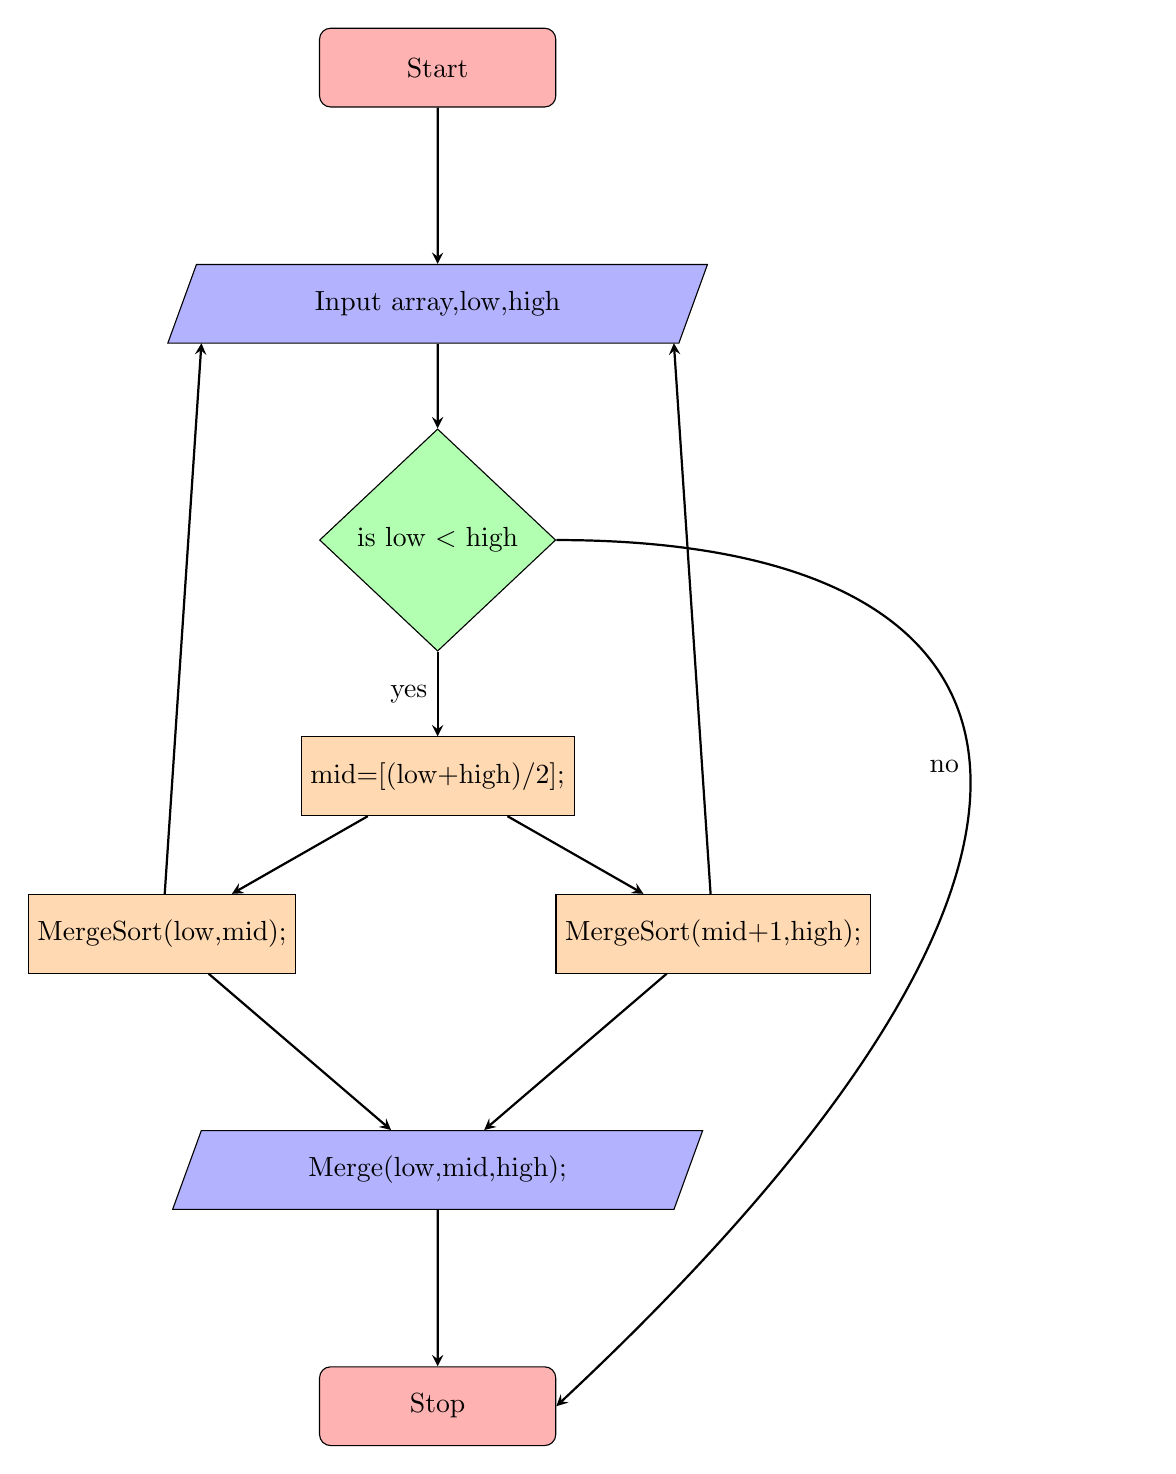
\begin{tikzpicture}[node distance=3cm]
\node (start) [startstop] {Start};
\node (in1) [io, below of=start] {Input array,low,high};
\node (dec1) [decision, below of=in1] {is low $<$ high};
\node (ou1) [process, below of=dec1] {mid=[(low+high)/2];};
\node (ou2) [process, below of=dec1, xshift=-3.5cm,yshift = -2cm] {MergeSort(low,mid);};
\node (ou3) [process, below of=dec1, xshift=+3.5cm,yshift = -2cm] {MergeSort(mid+1,high);};
\node (ou4) [io, below of=dec1,yshift = -5cm] {Merge(low,mid,high);};
\node (stop) [startstop, below of=ou4] {Stop};
\draw [arrow] (start) -- (in1);
\draw [arrow] (in1) -- (dec1);
\draw [arrow] (dec1) -- node[anchor=east] {yes}(ou1);
\draw [arrow] (dec1.east) ..controls (8,-6) and (9,-10).. node[anchor=east] {no}(stop.east);
\draw [arrow] (ou2) -- (-3,-3.5)(in1);
\draw [arrow] (ou3) -- (+3,-3.5)(in1);
\draw [arrow] (ou1) -- (ou2);
\draw [arrow] (ou1) -- (ou3);
\draw [arrow] (ou2) -- (ou4);
\draw [arrow] (ou3) -- (ou4);
\draw [arrow] (ou4) -- (stop);
\end{tikzpicture}
\end{center}
\pagebreak

\section{Example Program}

The following Python program sorts a list of numbers using the divide and conquer approach.

\begin{lstlisting}[language=Python]
def merge_sort(array):
  if len(array) <= 1:
    return array

  middle = len(array) // 2
  left = merge_sort(array[:middle])
  right = merge_sort(array[middle:])

  return merge(left, right)

def merge(left, right):
  merged = []
  i = 0
  j = 0

  while i < len(left) and j < len(right):
    if left[i] <= right[j]:
      merged.append(left[i])
      i += 1
    else:
      merged.append(right[j])
      j += 1

  merged += left[i:]
  merged += right[j:]

  return merged

if __name__ == "__main__":
  array = [10, 5, 2, 1, 8, 7, 6, 3, 4, 9]
  sorted_array = merge_sort(array)
  print(sorted_array)

\end{lstlisting}

\section{Conclusion}

Divide and conquer is a powerful problem-solving approach that can be used to solve a wide variety of problems. This approach is often used to solve problems that can be expressed in terms of a recursive relationship. The divide and conquer approach can be used to solve problems more efficiently than other approaches, such as brute force.

\end{document}
